%% --------------------------------------------------------------
%%
%% I N T R O D U C T I O N
%%
%% --------------------------------------------------------------
\section{Introduction}


\begin{frame}{}  %% ---------- Intro/motivation 
    \begin{tikzpicture}[overlay,remember picture]
        
        \uncover<1->{ % <-> |
            \node (t1) [anchor=center,scale=1,opacity=1] at ([shift={(-3.0cm,-0.20cm)}]current page.center){
                \parbox{0.7\textwidth}{
                    Binary Neutron Star (BNS) and Neutron Star Black Hole (NSBH) mergers expose 
                    properties of matter at densities much many times the nuclear saturation density. \\
                    \textbf{Multimessenger sources}
                    \begin{itemize}
                        \item Gravitational Waves (GWs)
                        \item Neutrino emission
                        \item Gamma-ray burst: emission from internal processes within a jet
                        \item Kilonova (kN): thermal radiation from decay of newly produced heavy nuclei
                        \item \textbf{GRB afterglow}: synchrotron (non-thermal) emission produced by GRB ejecta sweeping-up ISM
                        \item \textbf{Kilonova afterglow}: -//- by Kilonova ejecta sweeping up ISM
                    \end{itemize}
                    Numerical relativity simulations $\rightleftarrows$ EM transient models
            }};
            
        }
%            \uncover<1->{ % <-> |
%        \node (t1) [anchor=center,scale=1,opacity=1] at ([shift={(-3.5cm,-0.5cm)}]current page.center){
%            \parbox{0.6\textwidth}{
%                \begin{itemize}
%                    \item One of the ways to understand the properties of matter at supernuclear densities 
%                    is to study EM signatures of BNS, NSBH mergers and CCSNe. 
%                    %
%                    \item Non-thermal EM signatures: GRBs, kN afterglows, ... 
%                    %
%                    \item Origin: interaction between transrelativistic ejecta and ISM. 
%                    %
%                    \item Thus study of GRBs, kN probe the ejecta properties and by extension, the 
%                    properties of the postmerger/post-SNe remnant. 
%                    \item NR simulations + observations show 
%                \end{itemize}
%        }};
%        
%    }
        \uncover<1-1>{ % <-> |
            \node (img1) [anchor=center,scale=1,opacity=1] at ([shift={(5.6cm,-0.8cm)}]current page.center){
                \parbox{0.5\textwidth}{
                    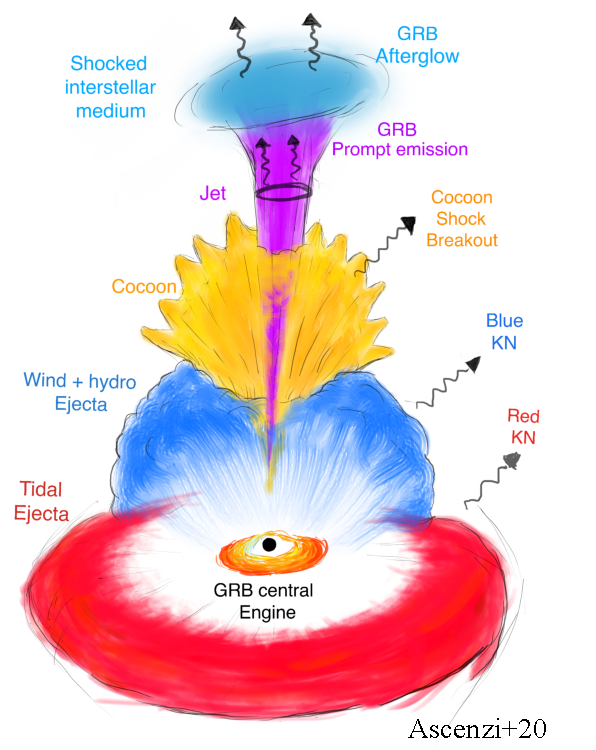
\includegraphics[height=7.0cm]{figures/Ascenzi20_EjectaEMPicture.pdf}
                    
                    %\small{\textbf{Artist depiction of ejecta$^\text{\citep{Ascenzi:2020xqi}}$}}
            }};
        }
    \end{tikzpicture}
\end{frame}

% =============================================================================================

\section{Observations}
\begin{frame}{}  %% ---------- Intro/motivation 
    \begin{tikzpicture}[overlay,remember picture]
        \uncover<1->{ % <-> |
            \node (t1) [anchor=center,scale=1,opacity=1] at ([shift={(-0.5cm,3.2cm)}]current page.center){
                \parbox{1.0\textwidth}{
                    No unambigous detection of GRB + kN afterglows. \\
                    Possible candidates: GRB160821B and \GRB{}. There is hope. \\
                    %
                    \GRB{}:
                    \begin{itemize}
                        \item shallow rising light cruve: structured, off-axis (dimm) 
                        \item late time flattening: lateral spreading, emergence of another component (spectral evolution)
%                        \textit{harder radio-to-X-ray spectrum} (lower $p$)
%                        \item Radio obs. $\rightarrow$ optically thin spectrum
%                        \item Lower $p=2$ \textit{is expected} in non-relativistic shocks (but with lower $\varepsilon_e$ as well)
                    \end{itemize}
            }};
        }
%        \uncover<1->{ % <-> |
%        \node (t1) [anchor=center,scale=1,opacity=1] at ([shift={(-5.5cm,0.7cm)}]current page.center){
%            \parbox{0.4\textwidth}{
%                No unambigous detection of GRB + kN afterglows. Possible candidates: GRB160821B and \GRB{}.
%                GRB170817 from [Hajela et al 2021]:
%                \begin{itemize}
%                    %                        \item late-time cahnge in afterglow (not a jet)
%                    \item Statistical fit indicates
%                    \textit{harder radio-to-X-ray spectrum} (lower $p$)
%                    \item Radio obs. $\rightarrow$ optically thin spectrum
%                    \item Lower $p=2$ \textit{is expected} in non-relativistic shocks (but with lower $\varepsilon_e$ as well)
%                \end{itemize}
%                
%        }};
%        }
        \uncover<1-1>{ % <-> |
            \node (img1) [anchor=center,scale=1,opacity=1] at ([shift={(-4.2cm,-1.8cm)}]current page.center){
                \parbox{0.5\textwidth}{
                    \GRB{} \\
                    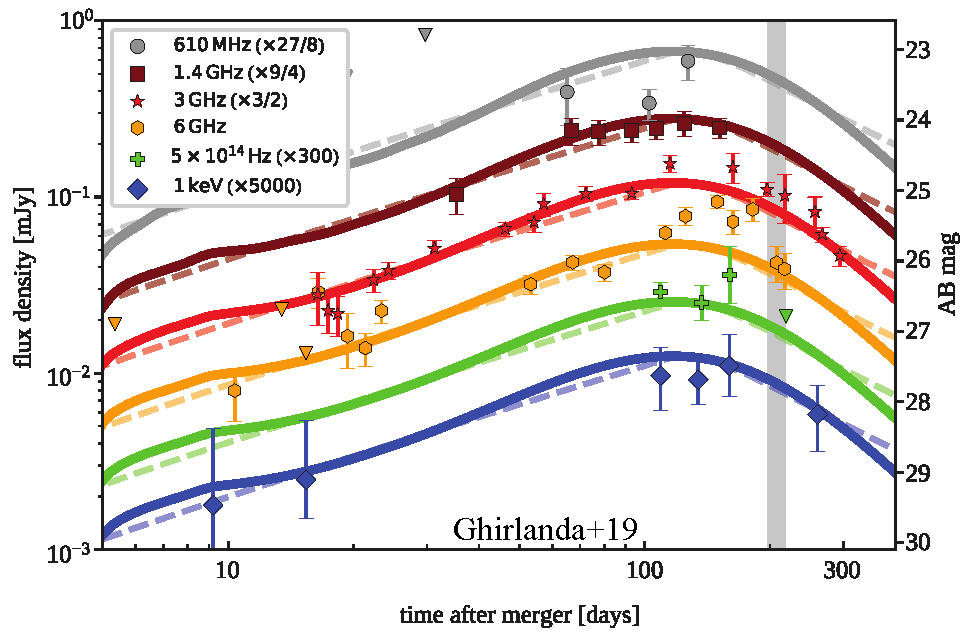
\includegraphics[height=4.0cm]{figures/Ghirlanda19_GRB170817A.pdf}
            }};
        }
        \uncover<1-1>{ % <-> |
            \node (img1) [anchor=center,scale=1,opacity=1] at ([shift={(1.5cm,-1.8cm)}]current page.center){
                \parbox{0.5\textwidth}{
                    \GRB{} \\ 
                    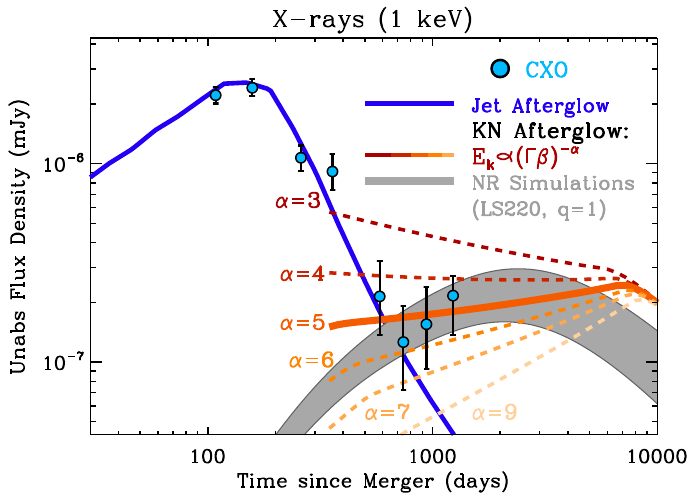
\includegraphics[height=4.0cm]{figures/Hajela21_ChangeGW170817-1.png}
            }};
        }
        \uncover<1-1>{ % <-> |
            \node (img1) [anchor=center,scale=1,opacity=1] at ([shift={(7.0cm,-1.8cm)}]current page.center){
                \parbox{0.5\textwidth}{
                    GRB160821B \\
                    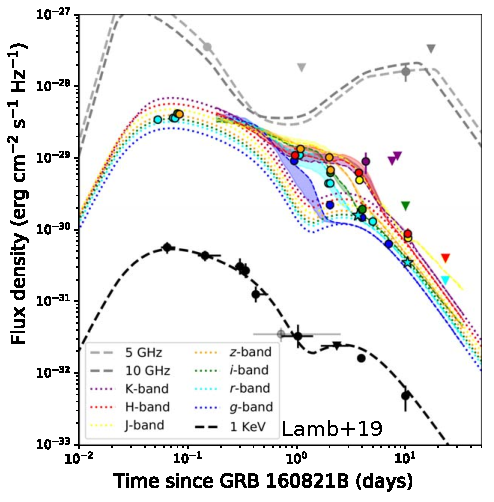
\includegraphics[height=4.02cm]{figures/Lamb19_GRB160821B.pdf}
            }};
        }
    \end{tikzpicture}
\end{frame}


% =============================================================================================

\section{NR simulations}
\begin{frame}{}  %% ---------- Intro/motivation 
    \begin{tikzpicture}[overlay,remember picture]
        \uncover<1->{ % <-> |
            \node (t1) [anchor=center,scale=1,opacity=1] at ([shift={(-3.7cm,2.5cm)}]current page.center){
                \parbox{0.60\textwidth}{
                    Simulations show 
                    \begin{itemize}
                        \item the fastest ejecta produced at \textit{core bounces}
                        \item ejecta properties depend in the binary parameters
                        \item ejecta is velocity \& laterally structured
                    \end{itemize}
                    
%                    \textbf{Key Observables}: 
%                    \begin{itemize}
%                        \item $F_{\nu,p}\propto E n^{(p+1)/4}\beta^{(5p-7)/2}\varepsilon_e^{p-1}\varepsilon_B^{(p+1)/4}D_L^{-2}\nu^{(-p-1)/2}$
%                        \item $t_{p}\propto E^{1/3} n^{-1/3} \beta^{-5/3}$
%                        %
%                        \item Timescale of years.
%                        %
%                        \item Trace the properties of the fastest ejecta
%                        %
%                    \end{itemize}
            }};
        }
        \uncover<1-1>{ % <-> |
            \node (img1) [anchor=center,scale=1,opacity=1] at ([shift={(4.1cm,-0.4cm)}]current page.center){
                \parbox{0.5\textwidth}{
                    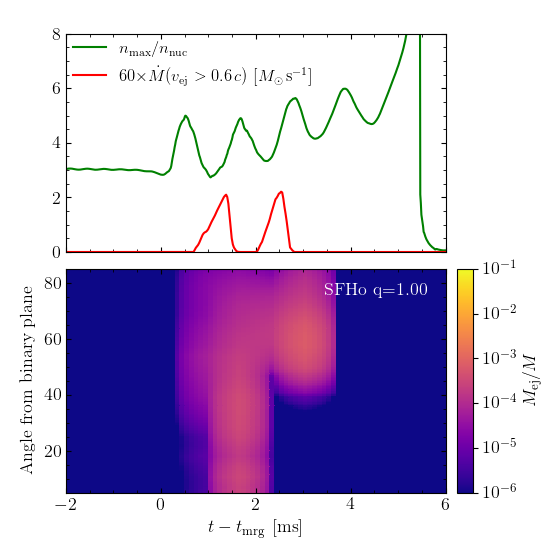
\includegraphics[height=7.6cm]{figures/SFHo_q100_LK_SR.png}
                    %\small{\textbf{Artist depiction of ejecta$^\text{\citep{Ascenzi:2020xqi}}$}}
            }};
        }
        \uncover<1-1>{ % <-> |
        \node (img1) [anchor=center,scale=1,opacity=1] at ([shift={(-2.6cm,-1.5cm)}]current page.center){
            \parbox{0.5\textwidth}{
                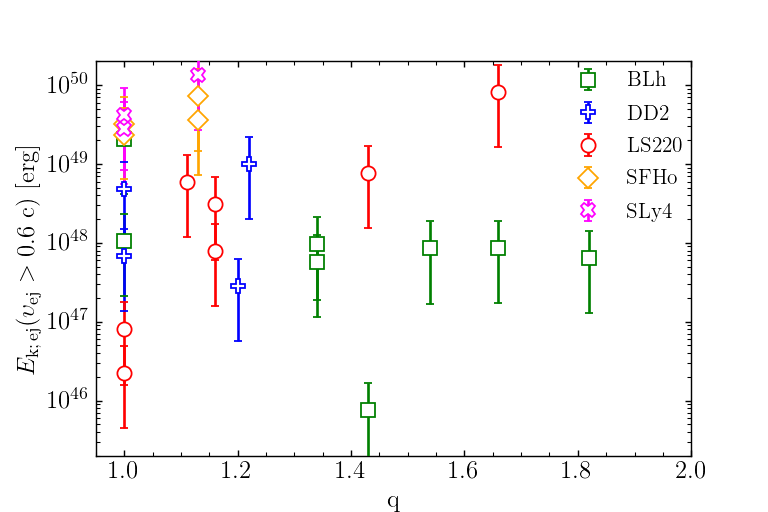
\includegraphics[height=4.6cm]{figures/scatter_ekej_vej06.png}
                %\small{\textbf{Artist depiction of ejecta$^\text{\citep{Ascenzi:2020xqi}}$}}
        }};
        }
    \end{tikzpicture}
\end{frame}

% =============================================================================================

\section{GRB-kN interaction}
\begin{frame}{}  %% ---------- Intro/motivation 
    \begin{tikzpicture}[overlay,remember picture]
        \uncover<1->{ % <-> |
            \node (t1) [anchor=center,scale=1,opacity=1] at ([shift={(-3.5cm,-0.5cm)}]current page.center){
                \parbox{0.5\textwidth}{
                    (i) GRB ejecta breaks out of kN ejecta (see \eg, Nativi+20)\\
                    (ii) kN ejecta polws through GRB ejecta 
                    \begin{itemize}
                        \item will kN ejecta catch up with GRB one and when?
                        \item how the GRB removing part of the ISM affects kN ejecta dynamics?
                        \item does it this interaction prodiuce an observable signature?
                    \end{itemize}
                }};
            
        }
        \uncover<1-1>{ % <-> |
            \node (img1) [anchor=center,scale=1,opacity=1] at ([shift={(4.5cm,-0.3cm)}]current page.center){
                \parbox{0.6\textwidth}{
                    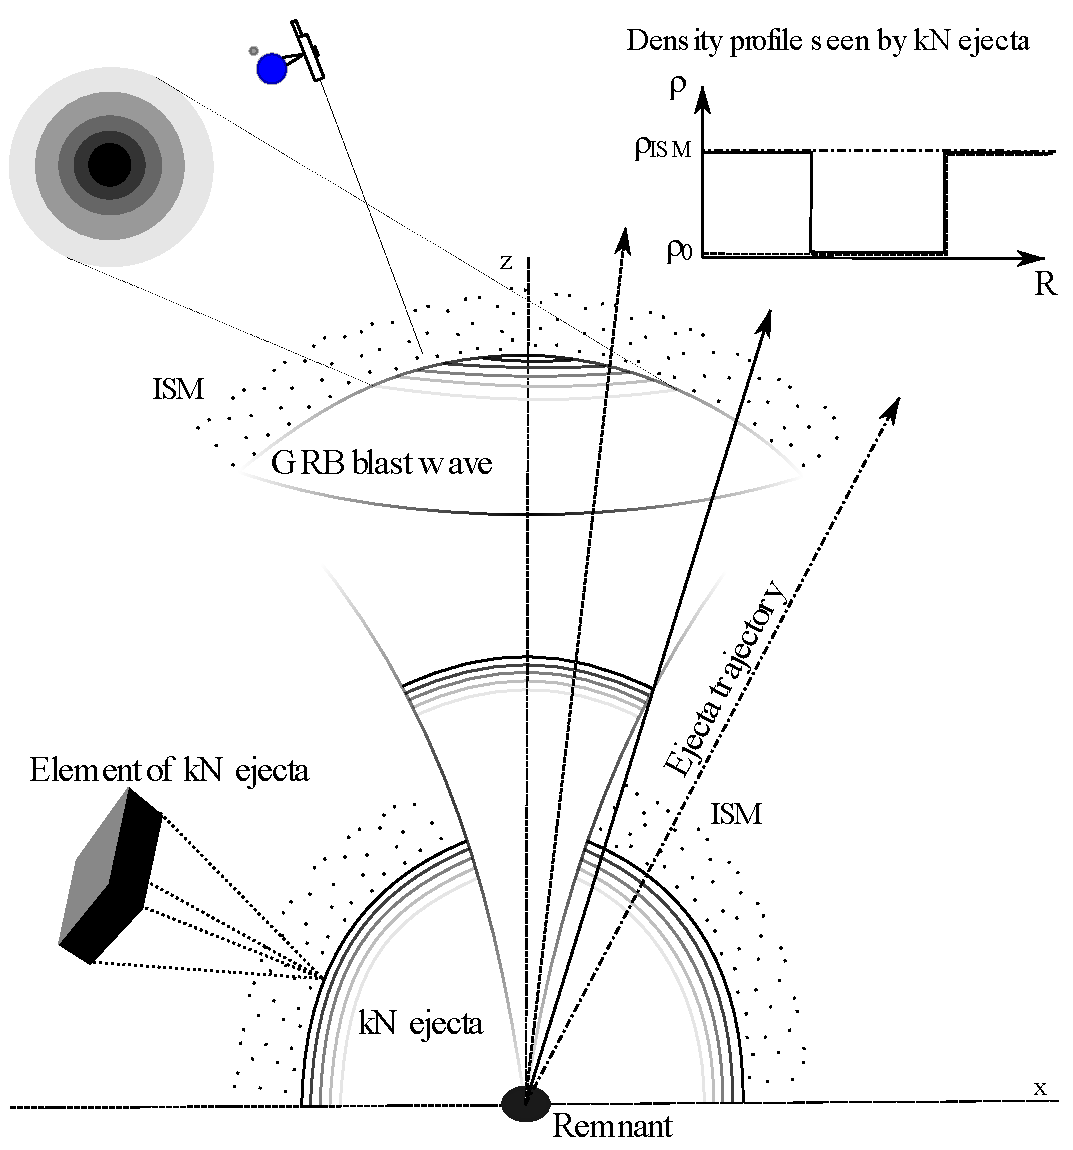
\includegraphics[height=7.8cm]{figures/structure2.pdf}
                    %\includesvg[height=7.2cm]{figures/structure2}
            }};
        }
    \end{tikzpicture}
\end{frame}



% =============================================================================================
\section{kN afterglows}
\begin{frame}{}  %% ---------- Intro/motivation 
    \begin{tikzpicture}[overlay,remember picture]
        \uncover<1->{ % <-> |
            \node (t1) [anchor=center,scale=1,opacity=1] at ([shift={(-3.1cm,-0.5cm)}]current page.center){
                \parbox{0.68\textwidth}{
                    \textbf{Main Features}:
                    \begin{itemize}
                        \item Synchrotron emission from mildly relativistic ejecta
                        (similar to GRB afterglow and SNe remnants)
                        %
                        \item Expected in sGRBs but have not observed$(^*)$
                        %
                        \item Complex ejecta structure/geometry $\rightarrow$ non-trivial EM signature
                        %
                    \end{itemize}
                    
                    \textbf{Key Observables}: 
                    \begin{itemize}
                        \item $F_{\nu,p}\propto E n^{(p+1)/4}\beta^{(5p-7)/2}\varepsilon_e^{p-1}\varepsilon_B^{(p+1)/4}D_L^{-2}\nu^{(-p-1)/2}$
                        \item $t_{p}\propto E^{1/3} n^{-1/3} \beta^{-5/3}$
                        %
                        \item Timescale of years.
                        %
                        \item Trace the properties of the fastest ejecta
                        %
                    \end{itemize}
            }};
        }
        \uncover<1-1>{ % <-> |
            \node (img1) [anchor=center,scale=1,opacity=1] at ([shift={(5.2cm,-4.2cm)}]current page.center){
                \parbox{0.5\textwidth}{
                    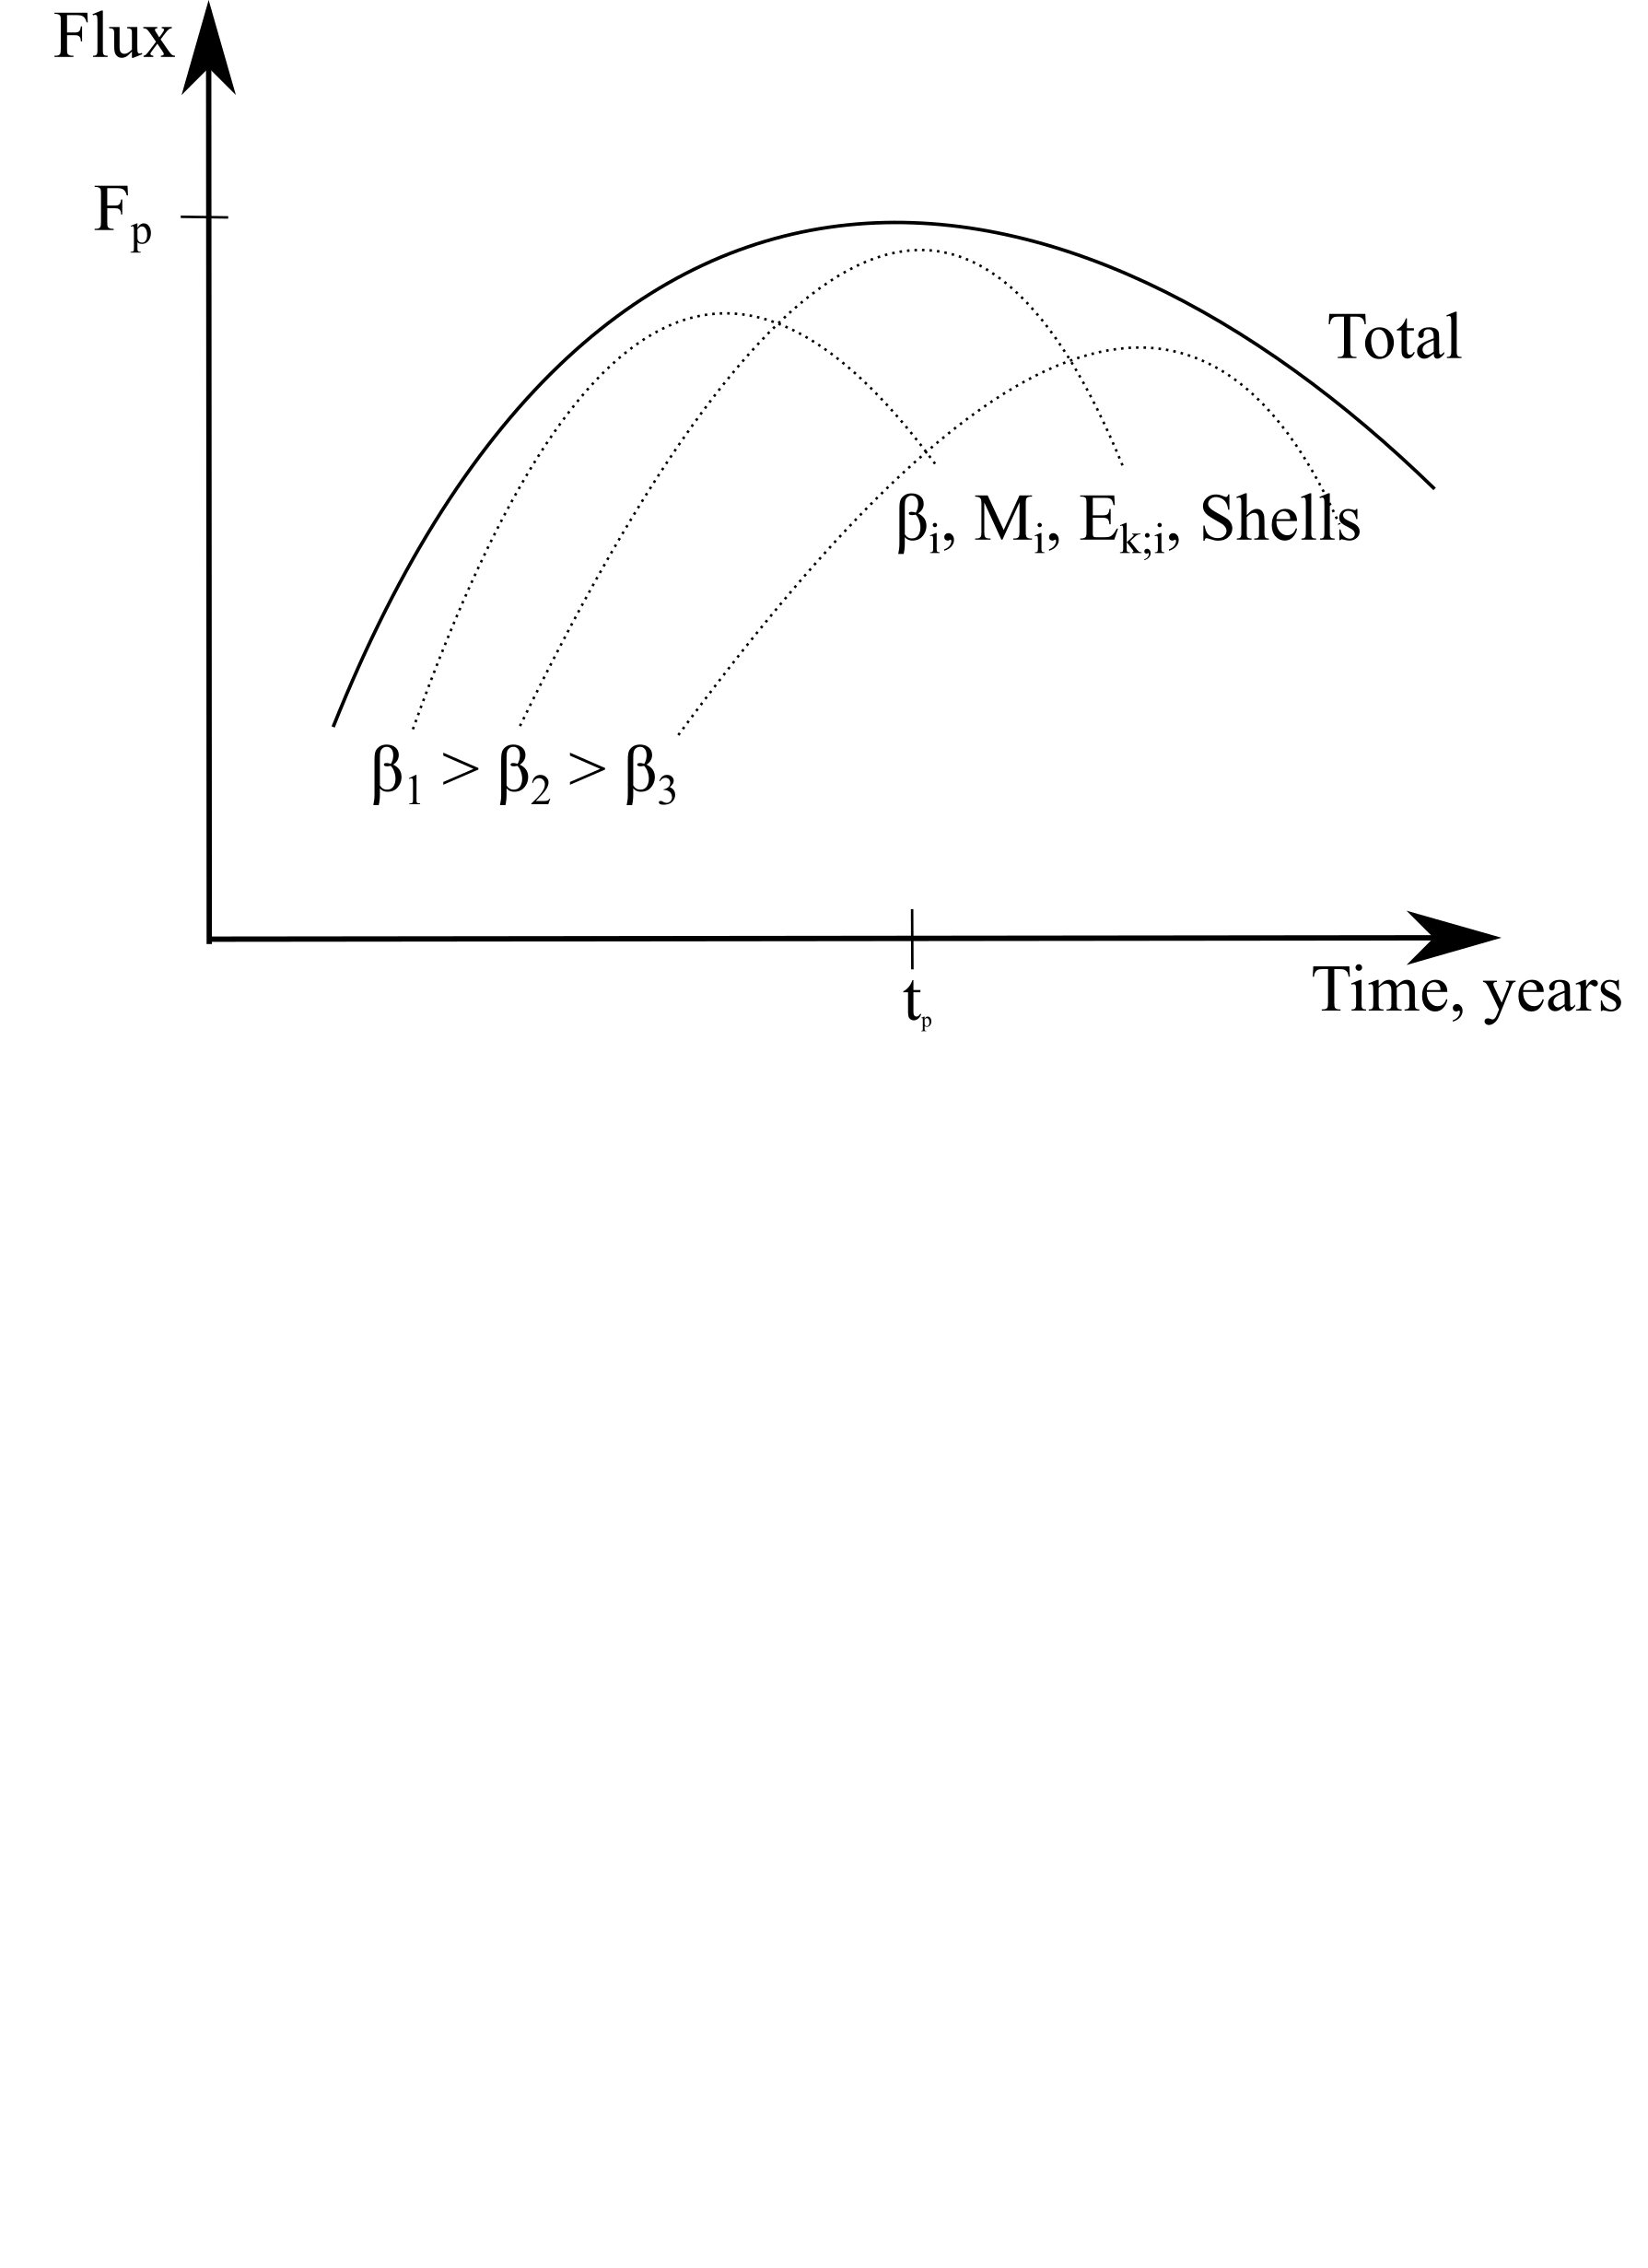
\includegraphics[height=8.6cm]{figures/afterglow_example.png}
                
                %\small{\textbf{Artist depiction of ejecta$^\text{\citep{Ascenzi:2020xqi}}$}}
            }};
        }
    \end{tikzpicture}
\end{frame}


% =============================================================================================

\section{Geometry}
\begin{frame}{}  %% ---------- Intro/motivation 
    \begin{tikzpicture}[overlay,remember picture]
        \uncover<1->{ % <-> |
            \node (t1) [anchor=center,scale=1,opacity=1] at ([shift={(-3.5cm,-0.5cm)}]current page.center){
                \parbox{0.5\textwidth}{
                    \textbf{Goal: combine structured GRB and kilonova afterglows}. \\
                    \textbf{Key features}:
                    \begin{itemize}
                        \item lateral structure \& lateral spreading of GRB ejecta
                        \item lateral \& velocity structure of kilonova ejecta
                        \item GRB jet evacuates ISM in front of ejecta
                        \item thermal electrons contribute to synchrotron emission from kilonova ejecta
                    \end{itemize}
            }};
            
        }
        \uncover<1-1>{ % <-> |
            \node (img1) [anchor=center,scale=1,opacity=1] at ([shift={(4.5cm,-0.3cm)}]current page.center){
                \parbox{0.6\textwidth}{
                    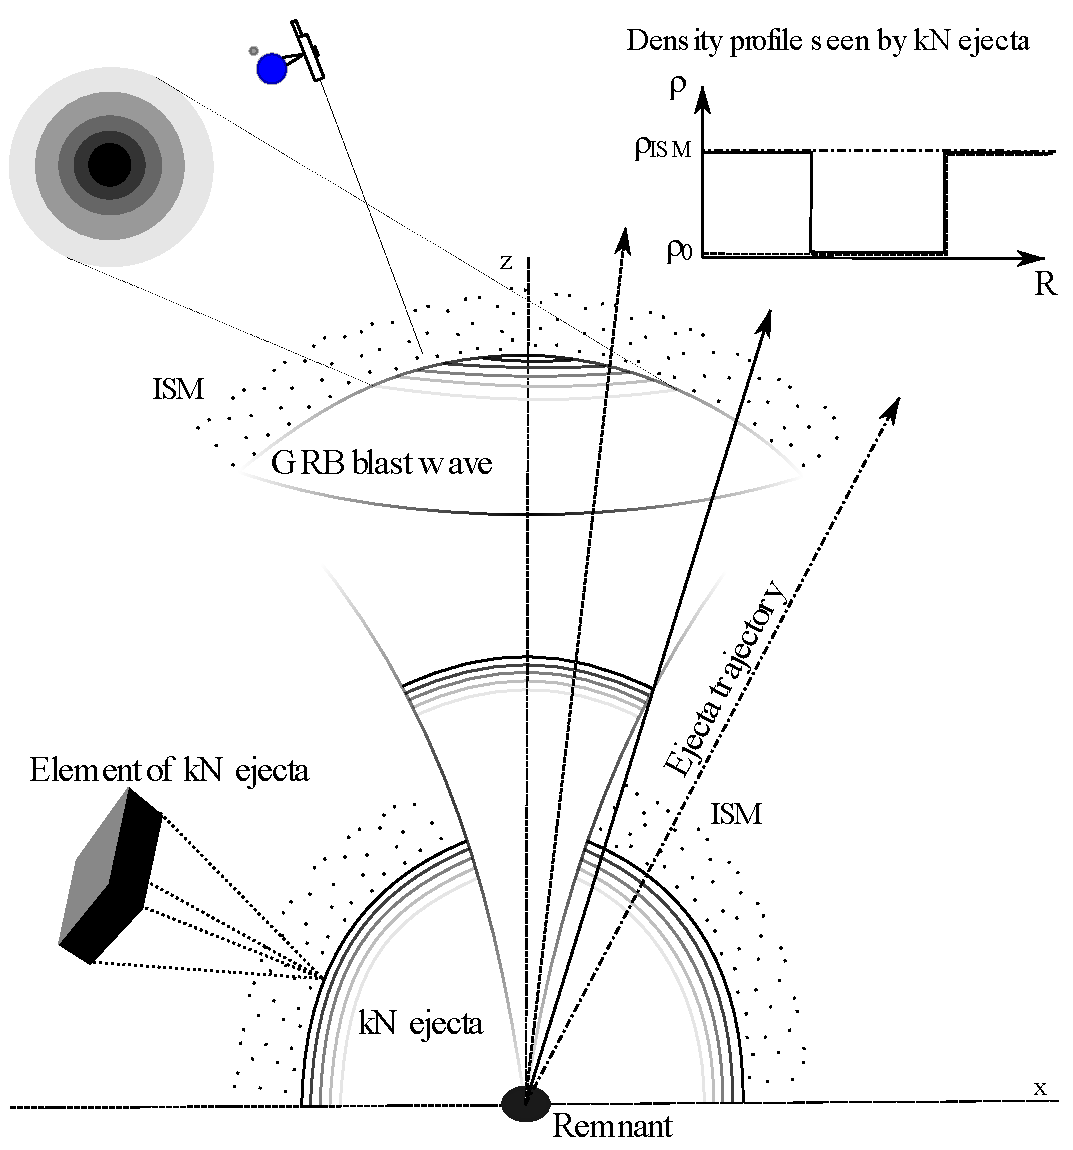
\includegraphics[height=7.8cm]{figures/structure2.pdf}
                    %\includesvg[height=7.2cm]{figures/structure2}
            }};
        }
    \end{tikzpicture}
\end{frame}



% =============================================================================================




%\section{Phsyics}
\subsection{Spectral evolution of GRB170817A}
\begin{frame}{}  %% ---------- Intro/motivation 
    \begin{tikzpicture}[overlay,remember picture]
        \uncover<1->{ % <-> |
            \node (t1) [anchor=center,scale=1,opacity=1] at ([shift={(-3.5cm,1.7cm)}]current page.center){
                \parbox{0.6\textwidth}{
                    GRB170817 from [Hajela et al 2021]:
                    \begin{itemize}
                        %                        \item late-time cahnge in afterglow (not a jet)
                        \item Statistical fit indicates
                        \textit{harder radio-to-X-ray spectrum} (lower $p$)
                        \item Radio obs. $\rightarrow$ optically thin spectrum
                        \item Lower $p=2$ \textit{is expected} in non-relativistic shocks (but with lower $\varepsilon_e$ as well)
                    \end{itemize}
                    
            }};
        }
        \uncover<1-1>{ % <-> |
            \node (img1) [anchor=center,scale=1,opacity=1] at ([shift={(5.0cm,0.1cm)}]current page.center){
                \parbox{0.5\textwidth}{
                    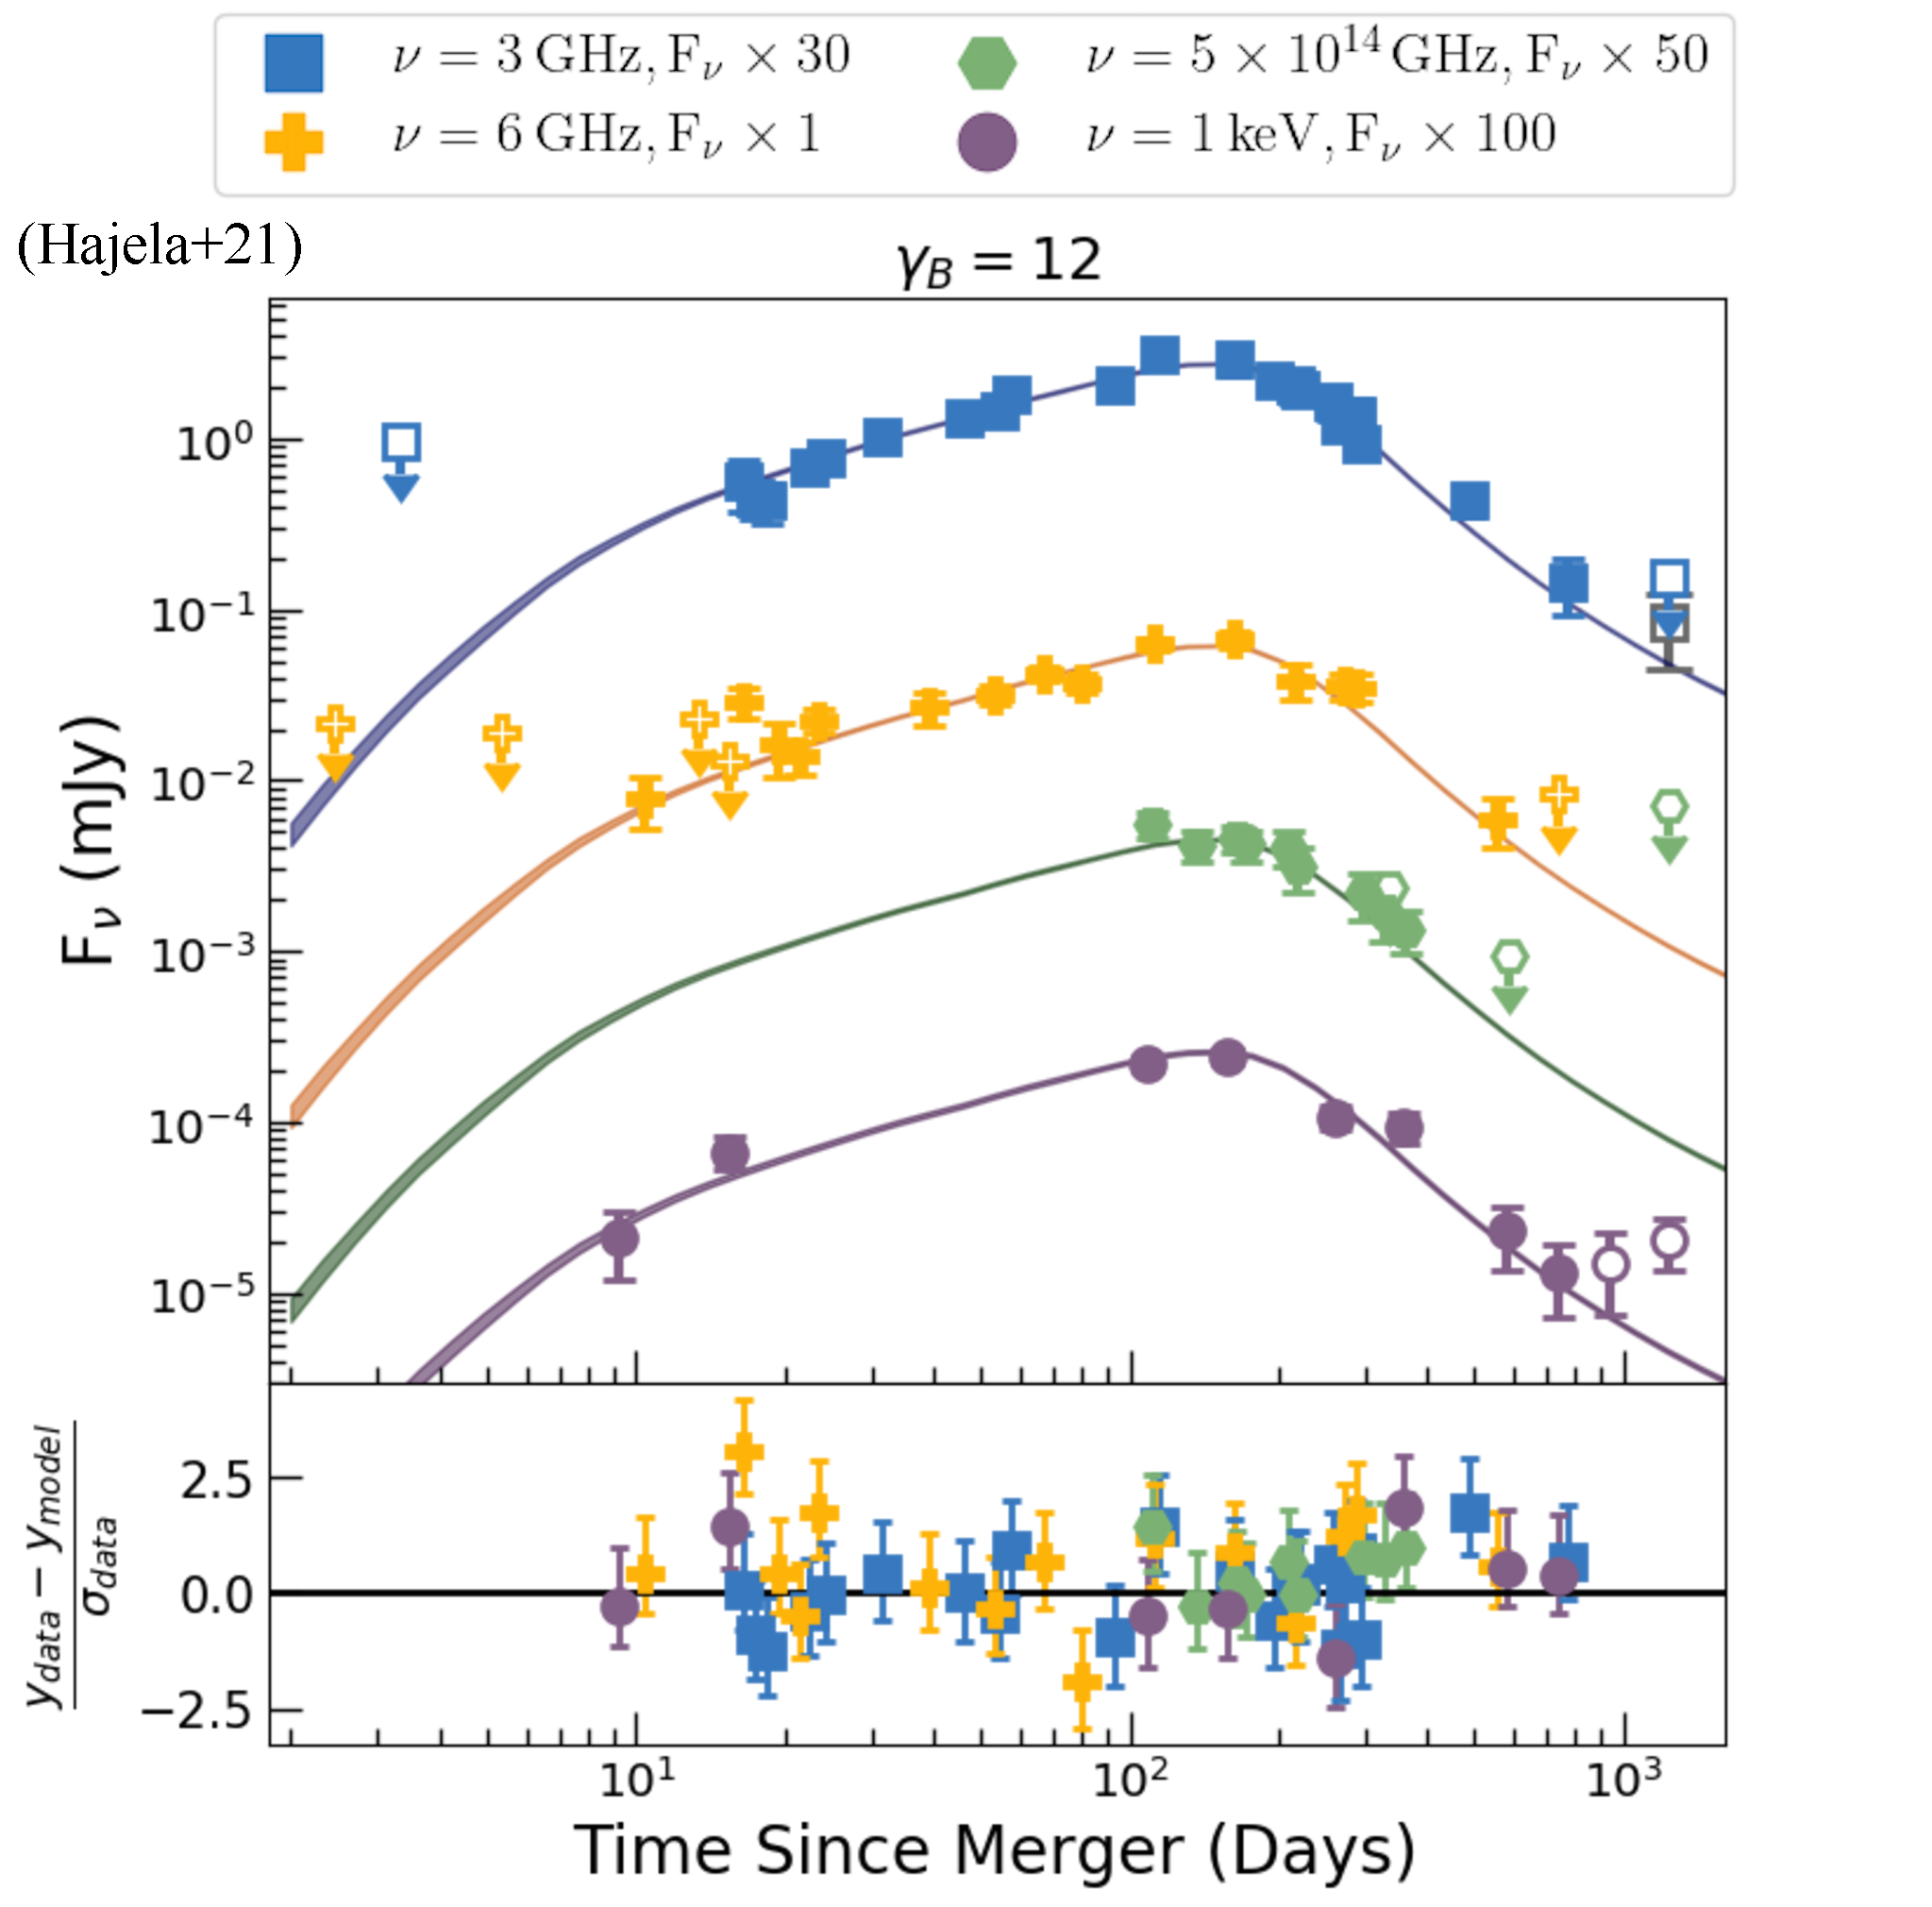
\includegraphics[height=6.5cm]{figures/figure4_2021paper.pdf}
            }};
        }
        \uncover<1-1>{ % <-> |
            \node (img1) [anchor=center,scale=1,opacity=1] at ([shift={(-3.0cm,-2.cm)}]current page.center){
                \parbox{0.5\textwidth}{
                    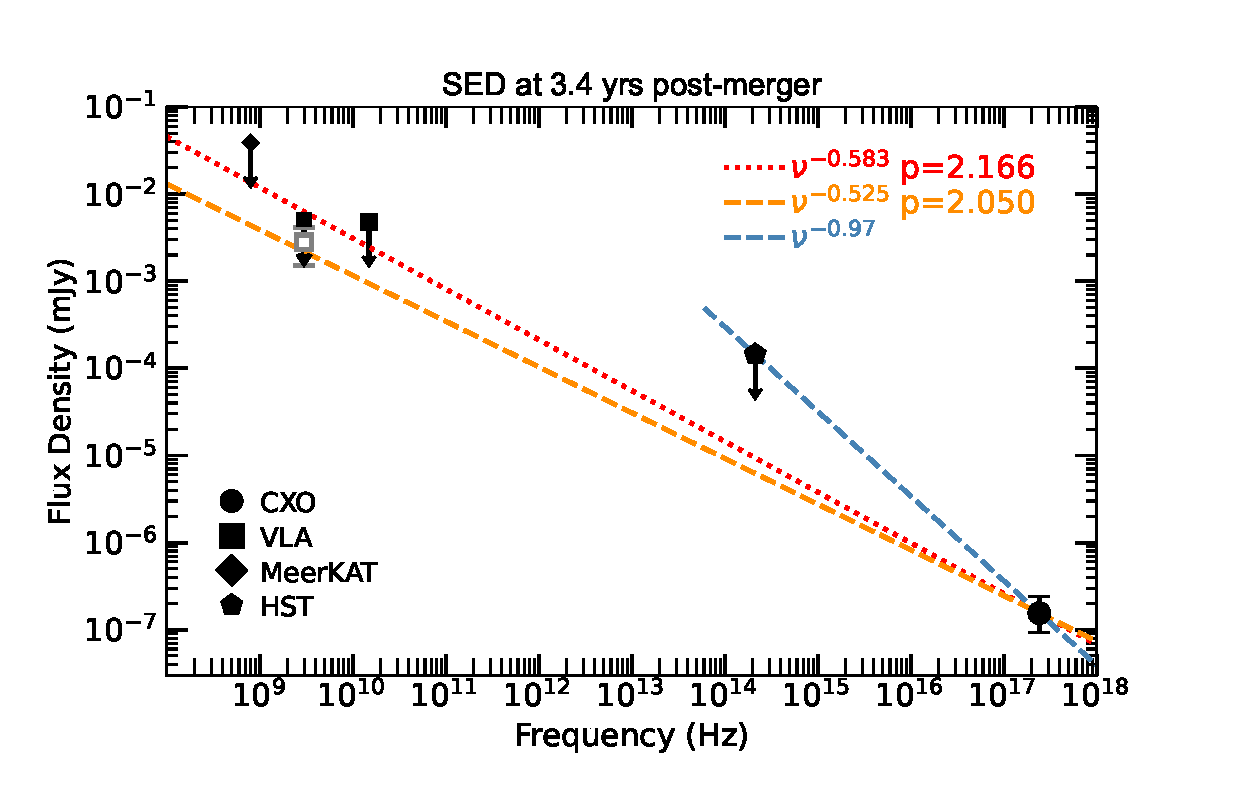
\includegraphics[height=4.5cm]{figures/SED1234days.eps}
            }};
        }
    \end{tikzpicture}
\end{frame}

